%----------------------------------------------------------------------------------------
%	PACKAGES AND OTHER DOCUMENT CONFIGURATIONS
%----------------------------------------------------------------------------------------


\documentclass[12pt,oneside,final,a4paper]{report}
\usepackage{generators/imports}
\makeglossaries

\renewcommand*{\acronymname}{List of Acronyms and Abbreviations}
\renewcommand{\glsnamefont}[1]{\textbf{#1}}

%Create acronyms here.
\newacronym{saas}{SaaS}{Software as a Service}
\newacronym{vcs}{VCS}{Version Control System}

%You can also do explanations.
\newglossaryentry{git}{name={Git},
    description={Git is a \gls{vcs} for tracking changes in computer files and coordinating work on those files among multiple people}}
\begin{document}
\begin{titlepage}

\newcommand{\HRule}{\rule{\linewidth}{0.5mm}} % Defines a new command for the horizontal lines, change thickness here

\center % Center everything on the page
 
%----------------------------------------------------------------------------------------
%	HEADING SECTIONS
%----------------------------------------------------------------------------------------

\textsc{\LARGE University of Bergen \\ Department of Informatics}\\[1.5cm] % Name of your university/college

%----------------------------------------------------------------------------------------
%	TITLE SECTION
%----------------------------------------------------------------------------------------

\HRule \\[0.5cm]
\begin{Huge}
	\bfseries{Title of your master thesis}\\[0.7cm] % Title of your document
\end{Huge}
\HRule \\[0.5cm]

%----------------------------------------------------------------------------------------
%	AUTHOR SECTION
%----------------------------------------------------------------------------------------

\large \emph{Author:} Your name\\
\large \emph{Supervisors:} Name of supervisors\\[2cm]

%----------------------------------------------------------------------------------------
%   LOGO SECTION
% 	This will require the graphicx package
%	Change the line to comment if you only want the UiB Logo
%	Logo for other faculties here: http://kapd.h.uib.no/profilmanual/99LastNed/99a_lastned.html
%----------------------------------------------------------------------------------------

\centerline{
\includegraphics[scale=1.9]{figures/canvasWithFaculty}}
%\centerline{
\includegraphics[scale=0.15]{figures/canvas}}  %change for your faculty

%----------------------------------------------------------------------------------------
%	DATE SECTION
%----------------------------------------------------------------------------------------

{\large \monthyeardate\today}\\[3cm] % Date, change the \today to a set date if you want to be precise

%----------------------------------------------------------------------------------------
%	LOGO SECTION
%----------------------------------------------------------------------------------------

\vfill % Fill the rest of the page with whitespace

\end{titlepage}
 % This is the titlepage
\begin{abstract}
Some abstract oart of your thesis
\thispagestyle{empty}
\end{abstract}
\newpage

{\tableofcontents \let\cleardoublepage\clearpage \listoffigures \let\cleardoublepage\clearpage \listoftables \let\cleardoublepage\clearpage \lstlistoflistings}
\pagenumbering{arabic}
\setcounter{page}{1}
\setlength{\parskip}{0.5cm plus4mm minus3mm}  

\chapter{Introduction}

Natum mucius vim id. Tota detracto ei sed, id sumo sapientem sed. Vim in nostro latine gloriatur, cetero vocent vim id. Erat sanctus eam te, nec assueverit necessitatibus ex, id delectus fabellas has.

Lorem ipsum dolor sit amet, iisque feugait quo eu, sed vocent commodo aliquid an. Minim suavitate dissentiet te eos. Dicunt eirmod adolescens no sed. Esse nonumy melius an mel, mei ut maiorum luptatum. Eu eum iudico scripta, movet option assueverit mel ex, mea at odio noluisse efficiendi. Ad vidisse atomorum conceptam quo, saepe volumus philosophia eos eu, delenit conceptam no usu.

Vituperata sadipscing deterruisset ei mel, at qui nonumy blandit. Delectus dissentiet et sea, ut rebum regione numquam nam, cum ex augue constituto. Te per nihil semper. Posse voluptatum qui an, aliquando democritum disputando id quo, everti perpetua cu vim. Laudem fabellas mei an, eu reprimique quaerendum usu. Quidam prompta fabellas ne est.

\section{Background}

Lorem ipsum dolor sit amet, cu graecis propriae sea. Eam feugiat docendi an, ei scripta blandit pri. Nonumes delicata reprimique nam ut. Eu suas alterum concludaturque est, ferri mucius sensibus id sed~\cite{raftAlg}.

We can do glossary for acronymes and abriviations also: \gls{saas}. As you see the first time it is used, the full version is used, but the second time we use \gls{saas} the short form is used. It is also a link to the lookup.


\subsection{Listings}
You can do listings, like in Listing~\ref{ListingReference}
\begin{lstlisting}[caption={[Short caption]Look at this cool listing. Find the rest in Appendix~\ref{Listing}},label=ListingReference]
$ java -jar myAwesomeCode.jar
\end{lstlisting}

You can also do language highlighting for instance with Golang:
And in line~\ref{LineThatDoesSomething} of Listing~\ref{ListingGolang} you can see that we can ref to lines in listings.

\begin{lstlisting}[caption={Hello world in Golang},label=ListingGolang,escapechar=|]
package main

import "fmt"

func main() {
    fmt.Println("hello world") |\label{LineThatDoesSomething}|
}

\end{lstlisting}

\subsection{Figures}

Example of a centred figure
\begin{figure}[H]
    \centering
    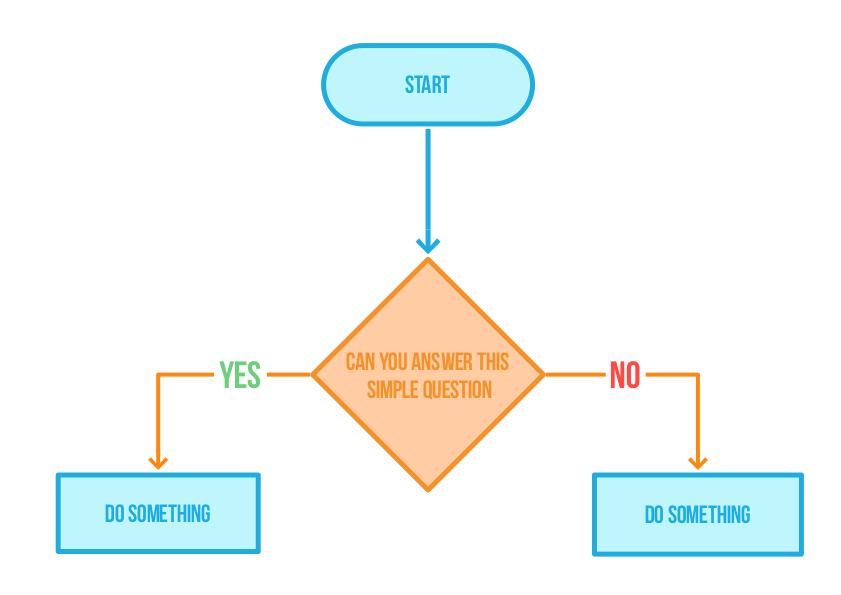
\includegraphics[scale=0.5]{figures/Flowchart}
    \caption{Caption for flowchart}
  	\medskip 
	\hspace*{15pt}\hbox{\scriptsize Credit: Acme company makes everything \url{https://acme.com/}}
    \label{FlowchartFigure}
\end{figure}

\subsection{Tables}

We can also do tables. Protip: use \url{https://www.tablesgenerator.com/} for generating tables.
\begin{table}[H]
\centering
\caption{Caption of table}
\label{TableLabel}
\begin{tabular}{|l|l|l|}
\hline
Title1 & Title2 & Title3 \\ \hline
data1  & data2  & data3  \\ \hline
\end{tabular}
\end{table}

\subsection{}
\chapter{Background}

This chapter aims to explain the basic concepts that are the most important to the work in this thesis.


% -------------------------------------------------------
% -------------------------------------------------------
% ----------------- Machine Learning --------------------
% -------------------------------------------------------
% -------------------------------------------------------
\section{Machine Learning}

The following sections will define the term 'Machine Learning'. 
It will describe some various ways that machine learning can be applied.



\subsection{What is machine learning?}

As a term, 'Machine Learning' is a subcategory if the umbrella term 'Artificial Intelligence'.
It is proposed as an alternative to traditional algorithms. 
Machine Learning takes a set of input (training) data, and attempts to reason about some quality of the input, 
without the author of the program explicitly telling the program what quality of the input data we are interested in reasoning about.
Instead, the author provides the Machine Learning model with their optimal target for the given input,
and the model must attempt to generalize over, and design its own algorithm to fit the target.

This approach has become useful in problems where discovering the target based on the model input becomes computationally intractible,
or when the target cannot be determined as a direct consequence of the input. 
An example of such a problem is sentiment analysis of text input. 
Given the sentence 'The nice boy made fun of the kind girl', 
it is difficult to design rules which can capture the sentiment of the sentence.
On one hand, the words 'nice', 'fun', and 'kind' indicate this sentence may have a positive sentiment.
In reality, our ability to reason tells us that this is not the case, and the sentence is of a negative nature.

Machine Learning is deeply rooted in Bayesian Statistics. (Noen gode setninger om bayes. Gjerne bayes teorem? Ikke mer enn et avsnitt. Dette er en AI-oppgave, ikke en statistikk-oppgave.)


\subsection{Linear Regression}

As a first study in the implementation of the concept 'Machine Learning', we look at Linear Regression.
To explan Linear Regression, we (tar for oss) an example in a two dimensional, euclidean space.

We are given a set of input data coordinates. 
Each coordinates consists two number a real number

$$  (x_i, y_i) \in X $$


weights
bias
\subsubsection{Loss}
loss



\subsection{Multi Layer Perceptron}
\subsection{Neural Networks}
underfitting and overfitting?
\subsubsection{Linear Layers}
\subsubsection{Activation functions}
\subsection{Backpropagation}
\subsection{Supervised and unsupervised learning}














% -------------------------------------------------------
% -------------------------------------------------------
% ---------------------- Graphs -------------------------
% -------------------------------------------------------
% -------------------------------------------------------
\section{Graphs}
\subsection{Nodes and Edges}
\subsection{Directed Acyclic Graphs}




% -------------------------------------------------------
% -------------------------------------------------------
% ---------------- Graph Neural Networks ----------------
% -------------------------------------------------------
% -------------------------------------------------------
\section{Graph Neural Networks}
\subsection{The Convolution Layer}
\subsection{Permutation invariance and equivariance}
\subsection{Attention and Message Passing}




% -------------------------------------------------------
% -------------------------------------------------------
% --------------- Gated Recurrent Units -----------------
% -------------------------------------------------------
% -------------------------------------------------------
\section{Gated Recurrent Units}
\subsection{Backpropagation Through Time}
\chapter{Project methodology and setup}

\section{The Geauvadis Dataset}


% Include more chapters as required.
%%=========================================

% Alternative 1 of printing glossaries & acronymes
%\renewcommand{\glossarypreamble}{\footnotesize}
%\printglossary[style=super, type=\glsdefaulttype] \let\cleardoublepage\clearpage
%\printglossary[style=super, type=\acronymtype]


%Alternative 2
%Simplified way of printing glossaries, slower than alt 1, but has better compatibility
\printnoidxglossaries

% Include more appendices as required.
%%=========================================
\clearpage
\DeclareRobustCommand{\VAN}[3]{#3}
\addcontentsline{toc}{chapter}{Bibliography}
\bibliographystyle{generators/myplainnat}
\bibliography{generators/refs}
\appendix
\titleformat{\chapter}[display]
  {\normalfont\large\bfseries}% <- font for label "Appendix A", default \huge
  {\chaptertitlename\ \thechapter}
  {20pt}
  {\large}% <- font for title, default \Huge

\chapter{Generated code from Protocol buffers}

\begin{lstlisting}[caption={Source code of something},label=Listing]
System.out.println("Hello Mars");
\end{lstlisting}
\end{document}
